\documentclass[conference]{IEEEtran}
\providecommand{\e}[1]{\ensuremath{\times 10^{#1}}}
\usepackage{times}
\usepackage[brazil,english]{babel}
\usepackage[utf8]{inputenc}
\usepackage[T1]{fontenc}
\usepackage{indentfirst}
\usepackage{amsmath,amssymb,amsthm}
\usepackage{graphicx,url,subfig}
\usepackage[table,xcdraw]{xcolor} % pacote extra para colocar cores nas celulas da tabel
\usepackage{tikz}
\usepackage{pgfplots}

\graphicspath{ {img/} }

\title{
\includegraphics[scale = 0.3]{GnuDebian.png}\\
	GNU Debian}

\author{	
\IEEEauthorblockN{Francisco Anderson Bezerra Rodrigues, Marcelo Bulhões Fonseca, Vitor Silva De Deus} \\
\IEEEauthorblockA{Departamento de Ciência da Computação, \\ Universidade de Brasília\\
%\IEEEauthorblockA{Email: anders1232@aluno.unb.br}
}
}

\begin{document} 

\maketitle
\selectlanguage{brazil}  

%\begin{abstract}
%Aqui vai o resumo do artigo! 

%\end{abstract}


\section{Introdução}\label{sec:intro}
Debian é um projeto e um sistema operacional iniciado em 16 Agosto de 1993 por Ian Murdock\cite{DebianHistory}. Cada versão possui o nome de um personagem de Toy Story. É uma distribuição utilizada por várias organizações pelo mundo\cite{DebianUsers} graças à sua estabilidade, que o torna ideal para servidores.

\section{Propósito do Debian}\label{sec:prop}
Debian é um sistema operacional com o objetivo de ser um sistema operacional completamente livre. No qual qualquer um pode baixar, modificar e compartilhar. De acordo com o projeto GNU~\cite{FreeSoftware}, um software para ser considerado livre, deve permitir que seus usuários possuam todas as seguintes liberdades fundamentais:
\begin{itemize}
	\item Liberdade para rodar o software da forma que o usuário quiser, e para qualquer propósito.
	\item Liberdade para estudar como o programa funciona, e poder editá-lo para que o programa compute da forma que o usuário quiser.
	\item Liberdade para redistribuir cópias.
	\item Liberdade para distribuir suas modificações para outras pessoas.
\end{itemize}
Para que essas liberdades sejam possíveis é necessário que o código fonte do software seja disponibilizado.

O Advanced Packaging Tool(APT) foi criado no projeto Debian e atualmente é usando em várias distribuições. Muitas delas baseadas no próprio Debian, como o Ubuntu e o Mint(que também possui uma versão baseada no Ubuntu).

\section{Requisitos de Aplicações}\label{sec:req}


\includegraphics[scale = 0.4]{Tux.png}\\
\section{Linux}\label{sec:linux}

\subsection{Arquitetura}\label{sec:LinuxArq}
O Linux é um kernel monolítico Unix-like criado por Linus Benedict Towards em 1991.\cite{LinuxHistory} Enquanto o GNU Project ficava fazendo tentativas de criar um kernel não monolítico(o que resultou no Hurd) o Linus conseguiu criar um kernel monolítico que era compatível com o sistema GNU. Desde então quase todos os esforços de desenvolvimento do kernel do sistema operacional GNU se voltaram para o Linux.\\

\subsection{Gerência de Memória}\label{sec:LinuxMem}

O linux usa segmentação-paginação para alocação de espaço em memória. Em sistemas Alpha AXP usa páginas de 8 kbytes e em sistemas Intel x86 usa páginas de 4kbytes. A cada uma dessas páginas é dado um único número, o PFN(page frame number)\cite{GerenciaMemLinux}.\\

Um endereço de memória virtual é composto de duas partes. Um offset e o numero de frame da página virtual. Cada processo possui uma tabela de páginas. Cada entrada nessa tabela contém as seguintes informações:\\

\begin{enumerate}
	\item flag de validade:indica se a entrada é válida
	\item O frame referente a pagina dessa entrada
	\item Informação de controle de acesso. Como a página deve ser usada e etc
\end{enumerate}
\cite{GerenciaMemLinux}
\\

Quando é necessário alocar novas páginas e não se tem espaços vazios o SO deve definir uma política para desalocar alguma página e colocar outra no lugar. O linux usa a política LRU(Least Recently Used). Nesse esquema, páginas pouco acessadas são boas candidatas para troca(swapping)\cite{GerenciaIOLinux}.

\subsection{gerência de E/S}\label{sec:LinuxES}
A getencia de entrada e saída no linux é realizada por um escalonador chamado CFQ(Complete Fair Queuing I/O Scheduler). O CFQ trata requisições de I\O baseado no processo que originou essa requisição, ou seja, cada processos possui filas independentes. As filas são ordenadas por tipo de requisição, requisições semelhantes ficam próximas O algoritmo de escalonamento utilizado nas filas é o round robin\cite{GerenciaIOLinux}.

\begin{figure}[h!]
	\centering
	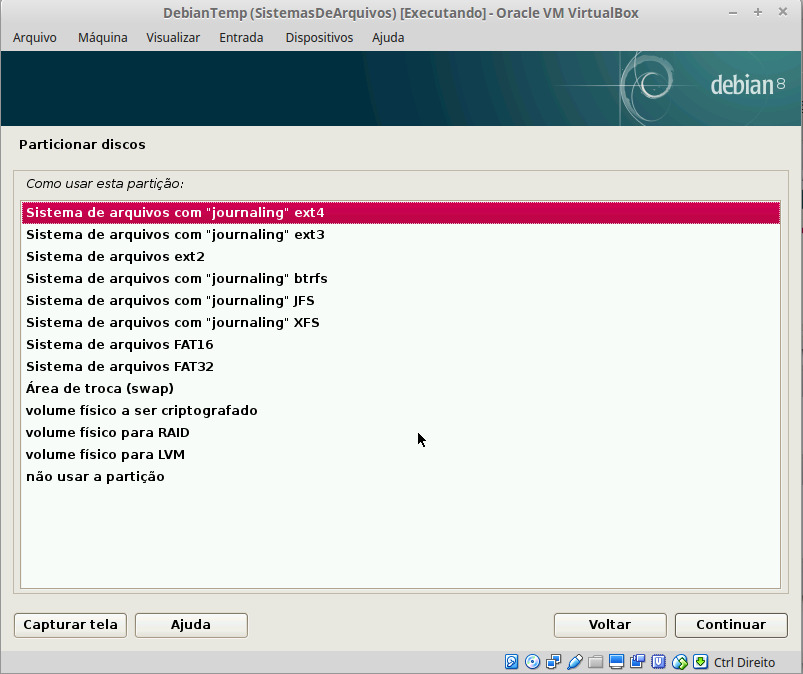
\includegraphics[scale=0.3]{SistemasArquivosLinux.jpeg}
	\caption{Tela de escolha de sistema de arquivo a ser instalado no Debian Linux.}
	\label{fig:SisAqrLinux}
\end{figure}
%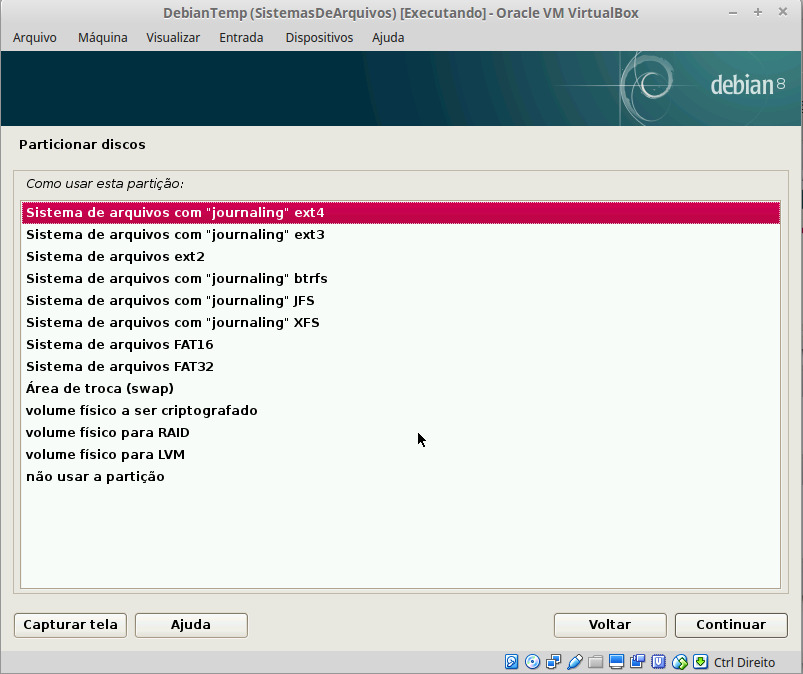
\includegraphics[scale = 0.27]{SistemasArquivosLinux.jpeg}
\subsection{gerência de Processos}\label{sec:LinuxPROC}

Os primeiros escalonadores do linux eram bastante simples, sem foco em arquiteturas massivas ou com muitos processadores multithread. O escalonador do linux 1.2 usava uma fila circular com Round-Robin. No linux 2.2 foi inserido outro escalonador com políticas de escalonamento para tarefas de tempo real, tarefas não preemptivas e tarefas de tempo não real, ou seja,  classes de escalonamento. Além disso também foi incluído suporte para SMP(symmetric multiprocessing)\cite{LinuxSchedulerIBM}.\\
\\
 No kernel 2.4 foi  inserido outro escalonador relativamente simples com complexidade O(n). Ele era relativamente ineficiente, limitava escalabilidade e era lento para processos de tempo real. Também se mostrou ruim para arquiteturas de multiprocessador. No kernel 2.6, introduziu-se o chamado de escalonador O(1), por ter complexidade O(1). Esse possuía suporte a SMP e cada fila de execução possuía dois arrays de prioridade.\\

 O array de tarefas ativas e o de expiradas. No caso, cada array contém uma fila de processos por nível de prioridade. Essas filas contém listas de processos prontos em cada nível de prioridade. Os  arrays de prioridade também contém mapas de bits para para descobrir eficientemente a maior prioridade entre as tarefas prontas no sistema sem precisar percorrer as filas. Achar a próxima tarefa a ser executada é simplesmente selecionar o próximo elemento nas listas.\\

 Dada uma prioridade, as tarefas são escalonadas com Roud Robin. Mantêm-se dois arrays de prioridade para cada processador, um para tarefas ativas e outro para expiradas. O de expiradas contém todas as tarefas da lista de execução associada que já exauriram o temporizador. Quando uma tarefa esgota o seu temporizador um novo tempo é atribuído antes dessa tarefa ser movida para o array de expirados. Recalcular todas as temporizações é tão simples quanto trocar o array de expirados pelo de não expirados porque os arrays são acessados apenas por ponteiro. Trocar os arrays é tão rápido quanto trocar dois ponteiros\cite{LinuxSchedulerMIT}.\\

 O escalonador O(1) era muito mais escalável e incorporou interatividade com várias métricas heurísticas para determinar se as tarefas eram IO-bound ou process-Bound. Apesar das vantagens o escalonador O(1) tornou-se pesado no kernel. A grande massa de código necessária para calcular heurísticas tornou-se difícil de manejar.\\

 A nova mudança veio por meio do algoritmo RSDL(Rotating Staircase Deadline Scheduler), proposto por Con Kolivas e foi incorporado a versão 2.6.21 do kernel linux. Depois, Ingo Molnar, o criador do escalonador O(1) desenvolveu um algoritmo CFS baseado nas mesmas ideias do trabalho de Kolivas. A principal idéia por trás do CSF é manter a justiça no provimento do processador aos processos. Para manter esse balanceamento, a quantidade de tempo designada a uma tarefa no CFS é chamada de virtual-runtime. Quanto menor for o "virtual-runtime" de uma tarefa maior a necessidade que essa tarefa tem de ser executada.\\
 
O CFS também possiu uma politica de justiça processos bloqueados(sleeper fainess) para processos que estão parados esperando por I/O tenham algum tempo para execução quando precisarem, por exemplo. Entretanto, ao invés de manter as tarefas em uma fila de espera, o CFS mantem uma árvore "red-black" ordenada por tempo.\\

Uma árvore "red-black" é uma árvore auto-balanceável, as operações na árvore ocorrem com complexidade O(log n), onde n é o número de nós da árvore. Nessa estrutura, tarefas com maior necessidade do processador(menor virtual-runtime) são armazenadas no lado esquerdo da arvore, e tarefas com menor necessidade de serem executadas do lado direito \cite{LinuxSchedulerIBM}. O escalonamento ocorre como a seguir:
\begin{enumerate}
	\item O nó mais a esquerda da árvore é escolhido e enviado à execução.
	\item Se o processo conclui sua execução ele é removido do sistema e da árvore
	\item Se o processo alcança seu tempo máximo de execução(quantum) ou é bloqueado(voluntariamente ou por interrupção), ele é reinserido na árvore baseado em seu novo "virtual-runtime".
	\item O novo nó mais a esquerda será escolhido repetindo a iteração\cite{LinuxSchedulerWiki}
\end{enumerate}



Outra alternativa moderna ao escalonador O(1) é o BFS(Brain fuck scheduler). Também desenvolvido por Con Kolivas, esse escalonador evita o uso de configurações e heurísticas Em alguns benchmarks apresenta desempenho levemente ou moderadamente maior que o CFS mas não chegou a tomar o seu lugar. Está presente em distribuições como Sabayon Linux\cite{LinuxSchedulerBFS}.
\cite{LinuxSchedulerWiki}

\subsection{Funcionamento de interrupções}\label{sec:LinuxInt}
Uma das principais tarefas do gerenciador de interrupções do linux é encaminhar as interrupções para o trecho de código correto no próprio gerenciador. Esse código deve entender a topologia do sistema. O linux utiliza um conjunto de ponteiros para estruturas de dados que contém os endereços das rotinas que tratam cada interrupção. Essas rotinas pertencem aos "drivers" dos dispositivos no sistema e é responsabilidade de cada driver requisitar a interrupção correta. Um vetor de ponteiros chamado irq\_action contém as referências para as estruturas de dados citadas anteriormente, as quais se chama irqaction. Cada irqaction contém informações sobre o gerenciamento dessa interrupção, incluindo o endereço da rotina correspondente de gerenciamento da interrupção. Visto que o número de interrupções e como as mesmas são gerenciadas varia entre as arquiteturas e sistemas, o gerenciador de interrupções do linux é dependente disso. Isso significa que o tamanho do vetor irq\_action varia dependendo da arquitetura ou sistema.\\

Quando a interrupção acontece, o Linux deve determinar a sua origem lendo o status da interrupção armazenado em um registrador em algum controlador programável de instruções de interrupções(isso é dependente de sistema e arquitetura). Depois traduzir a origem em uma posição do vetor irq\_action. Caso não exista alguma posição referente a determinada origem o kernel retorna um erro, caso contrário irá chamar a rotina contida em irqaction na dada posição de irq\_action. Ao fim, o driver do dispositivo é responsável por informar o kernel se a operação foi concluída com sucesso ou não\cite{InterruptsLinux}.

\subsection{Suporte a Threads}\label{sec:LinuxThreads}
O linux dá suporte a threads tratando-as como processos e escalonando-os juntamente. Um processo pode ser visto como uma thread mas
processos podem contem múltiplas threads que compartilham seus recursos\cite{LinuxSchedulerIBM}.
\subsection{Segurança}\label{sec:LinuxSec}
O Debian sempre tem pelo menos três versões em desenvolvimento: a unstable, a testing e a stable. E às vezes também tem a versão oldstable e oldoldstable. A versão unstable, também chamada de sid é aquela onde o desenvolvimento acontece, é muito pouco estável e nem tudo que é produzido vai para as outras versões.\\

A versão testing contém os pacotes que se mostraram com alguma estabilidade no unstable e que pelo menos conseguem ser compilados para a maioria das arquiteturas do Debian. No testing os pacotes passam por um processo de maturação até serem considerados bastante confiáveis. Quando o sistema testing como um todo chega a um estágio avançado de desenvolvimento ele é promovido a stable.\\

A versão stable é a principal versão do GNU Debian, é considerado muito estável pois os pacotes pertencentes à essa distribuição já passaram por exaustivos testes e se comprovaram estáveis e seguros.\\

A versão oldstable é a versão stable antes da versão testing ter se tornado a stable, ela tem foco em manter atualizações de segurança e é mantida por interessados em usar essa específica versão. A versão oldoldstable é a versão oldstable antes da stable se tornar oldstable, e tem o mesmo princípio de funcionamento da oldstable.\\

Os pacotes da versão stable passar por tanto tempo de teste que geralmente possuem versões consideradas antigas por alguns usuários. Esses usuários podem usar a versão testing sem muitos riscos. Tamanha estabilidade dos pacotes provê segurança ao sistema como um todo, considerado um dos melhores para ser usado em servidores\cite{DebianVersions}.\\



\includegraphics[scale = 0.2]{FreeBSD.png}\\
\section{kFreeBSD}\label{sec:BSD}

\subsection{Arquitetura}\label{sec:BSDArq}
O FreeBSD é um sistema operacional monolítico Unix-like descendente do sistema operacional BSD. Como esse sistema operacional é considerado livre, o Debian Project extraiu o kernel desse sistema operacional o colocou no sistema GNU Debian. Esse kernel é chamado de kFreeBSD, o que significa "kernel of FreeBSD".\cite{Debian-kFreeBSD-wiki}

\subsection{Gerência de Memória}\label{sec:BSDMem}
O FreeBSD usa uma política de troca de páginas ao estilo Last Recent Used(LRU)\cite{FreeBsdArc}

\subsection{Gerencia de arquivo}\label{sec:BSDArquivo}
O FreeBSD da suporte pra diversos sistemas de arquivos linux. entre eles estão Ext2, UFS,FAT16 e FAT32. Desde versões anteriores existe suporte ao ext2fs. O ext2 foi baseado no Unix File System(UFS) e uma solução ao design do minix filesystem.\\

O bloco no ext2fs é composto por setores de tamanho fixo 512 bytes, o tamanho do bloco é definido na formatação, podendo chegar a 1024, 2048 ou 4096 bytes e um superbloco apresenta tamanho 1024. \\ 
Para encontrar blocos livres o ext2fs faz o uso de mapa de bits. Utiliza-se também um mapa de bits para i-node.\\ 

O FreeBSD e, consequentemente o kFreeBSD, não possuem suporte completo ao ext3 nem ao ext4. Relativo ao ext3 o kFreeBSD contém suporte parcial, sem fazer uso do journaling que o ext3 tem. E em relação ao ext4 o FreeBSD tem suporte apenas para leitura.\cite{kFreeBSD-ext4}\\

\begin{center}
	\begin{tabular}{c|c|c|c|c}
		\hline
		 & Minix FS & Ext FS & Ext2 FS & Xia FS \\
		Max FS size & 64 MB & 2 GB & 4 TB & 2 GB \\
		Max file size & 64 MB & 2 GB & 2 GB & 64 MB \\
		Max file name & 16/30 c & 255 c &255 c & 248 c \\
		3 times support & No & No & Yes & Yes \\
		Extensible & No & No & Yes & No \\
		Var. block size & No & No & Yes & No \\
		Maintained & Yes & No & Yes & ?
%		\hline
	\end{tabular}
\end{center}

\subsection{gerência de E/S}\label{sec:BSDES}
Para gerenciar o acesso a dispositivos de entrada e saída, o FreeBSD no geral emprega o C-LOOK scheduler\cite{FreeBSD-Hybrid}. Que também é chamado de escalonamento "elevador", que trata os cilindros do disco como se fossem andares de um prédio. Porém a a variação que esse elevador funciona de forma circular para equalizar a frequência com a qual cada cilindro/andar é visitado.\\

Esse escalonamento consiste em organizar a fila em ordem de crescente offset de E/S, com isso tenta-se maximizar a transferência aumentando o número de E/S em uma busca no disco, desta forma o algoritmo não consegue assegurar “justiça” e resultar em starvetion de outros processos.
 
O SO não se restringe apenas a este escalonamente, isto pode depender do sistema de arquivo usado, como o caso do ZFS(Zfile System) que utiliza do seu próprio método de escalonamento. Podendo assim fazer uso de outros metodos. \\

\begin{figure}[h!]
	\centering
	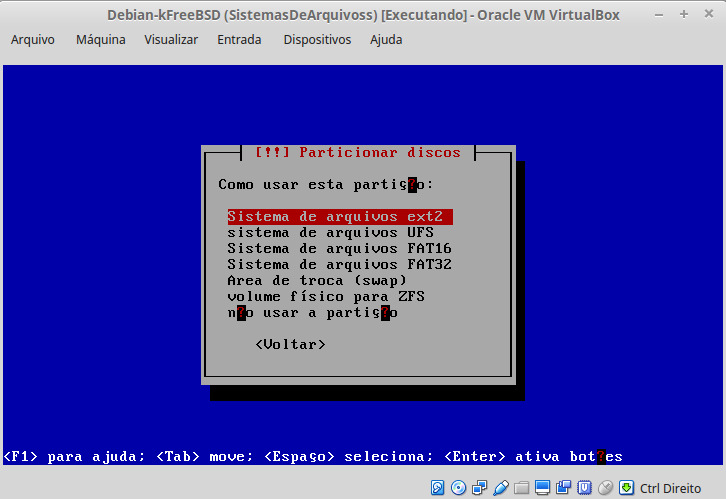
\includegraphics[scale=0.34]{SistemasArquivoskFreeBSD.jpeg}
	\caption{Tela de escolha de sistema de arquivo a ser instalado no Debian kFreeBSD.}
	\label{fig:SisAqrLinux}
\end{figure}
%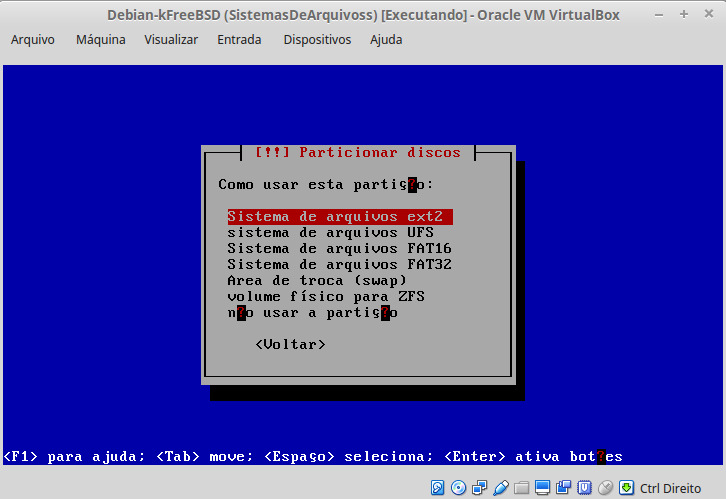
\includegraphics[scale = 0.27]{SistemasArquivoskFreeBSD.jpeg}

\subsection{gerência de Processos}\label{sec:BSDPROC}
FreeBSD trabalha com o escalonador de processos ULE, o ULE segue um estilo tradicional com filas de execução e fazendo uso de time slice. Tenta ser justo mas pode favorecer mais os processos interativos, o que o diferencia do CFS(escalonador usado no linux). Isso se dá ao uso baseado em filas multiníveis de tempo compartilhado, o algoritmo  separa os processos em threads e os classifica pra poder dar prioridade ao tipo do processo. Assim, os processos que usam todo o time slice têm sua prioridade diminuída e os processos que fazem tempo que não são rodados têm sua prioridade aumentada para evitar starvation.\\

O FreeBSD também dá suporte a aplicações de tempo real, mantendo essas aplicações numa fila diferente da fila dos outros processos.\cite{DesignImplementationFreeBSD}\\ \\



\subsection{Funcionamento de interrupções}\label{sec:BSDInt}

\subsection{Suporte a Threads}\label{sec:BSDThreads}
o FreeBSD poddui suporte a threads POSIX(Portable Operation System Interface). Seu escalonador trabalha com threads, o que implica em que as threads funcionam no nível de núcleo.\cite{DesignImplementationFreeBSD}

\subsection{Segurança}\label{sec:BSDSec}
Como o GNU Debian Linux, o GNu Debian kFreeBSD também possui versões oldstable e stable. E também recebe atualizações de segurança pela equipe de segurança do Debian.\cite{DebiankFreeBSDVersions}\\

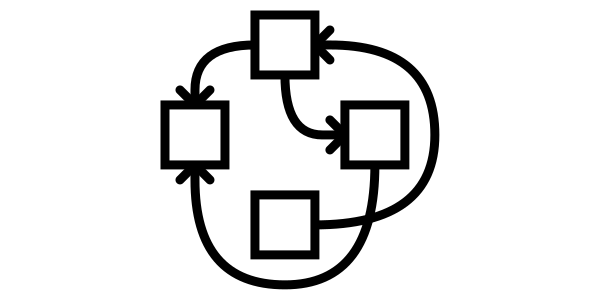
\includegraphics[scale = 0.5]{Hurd.png}\\
\section{Hurd}\label{sec:Hurd}

\subsection{Arquitetura}\label{sec:HurdArq}
O kernel GNU/Hurd possui a arquitetura cliente/servidor e faz uso de microkernels os quais podem executar instruções privilegiadas. O microkernel instalado por padrão é o GNU/Mach. Porém existem outros microkernels que ao longo do tempo tentaram-se colocar no Hurd, como por exemplo o L4, Coyotos e o Viengoos. No Hurd, pode-se atrelar à arquivos, máquinas de tradução. Que podem prover diversas funcionalidades, como por exemplo implementar o protocolo ftp de forma transparente, prover gerenciamento de histórico de arquivos entre outras coisas muito interessantes.\cite{HurdPaper}

\subsection{Gerência de Memória}\label{sec:HurdMem}

\subsection{gerência de Processos}\label{sec:HURDPROC}

\subsection{gerência de E/S}\label{sec:HurdES}
No GNU/Hurd as operações de entrada e saída são feitas com o uso de portas de comunicação que implementam pelo menos o protocolo de arquivo ou o protocolo de socket. As operações são realizadas a partir de chamadas de procedimento remoto(RPC's) nessas portas de comunicação\cite{HurdIO}.

\begin{figure}[h!]
	\centering
	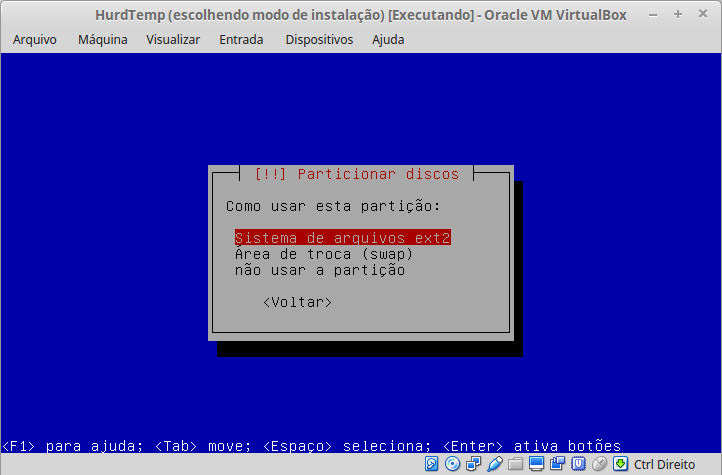
\includegraphics[scale=0.35]{SistemasArquivosHurd.jpeg}
	\caption{Tela de escolha de sistema de arquivo a ser instalado no Debian kFreeBSD.}
	\label{fig:SisAqrLinux}
\end{figure}
%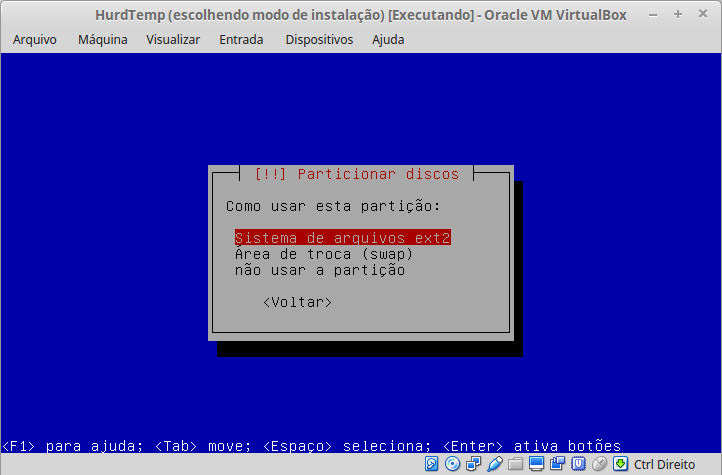
\includegraphics[scale = 0.27]{SistemasArquivosHurd.jpeg}

\subsection{Funcionamento de interrupções}\label{sec:HurdInt}

\subsection{Suporte a Threads}\label{sec:HurdThreads}
O GNU/Hurd faz uso agressivo de Threads como o objetivo de extrair o máximo do hardware.\cite{Hurd} Todas as bibliotecas do GNU/Hurd são thread-safe, ou seja, chamadas concorrentes aos serviços da biblioteca não fazem ela se comportar de forma inesperada.

\subsection{Segurança}\label{sec:HurdSec}
Um dos objetivos do Hurd é minimizar a quantidade de código que é executada no modo kernel através do uso de microkernel GNU Mach. O que aumenta a confiabilidade do sistema como um todo.\\

Porém, como o Hurd possui uma escassez crônica de denvolvedores, ele apenas possui a versão unstable. Ou seja, o GNU Debian Hurd não possui uma versão estável.

\bibliographystyle{unsrt}
\bibliography{arquivo.bib}
%\end{multicols*} %fim do texto em 2 duas colunas

\end{document}
